%%%%%%%%%%%%%%%%%%%%%%%%%%%%%%%%%%%%%%%%%%%%%%%%%%%%%%%%%%%%%%%%%
%%% %
%%% % weiiszablon.tex
%%% % The Faculty of Electrical and Computer Engineering
%%% % Rzeszow University Of Technology diploma thesis Template
%%% % Szablon pracy dyplomowej Wydziału Elektrotechniki 
%%% % i Informatyki PRz
%%% % June, 2015
%%%%%%%%%%%%%%%%%%%%%%%%%%%%%%%%%%%%%%%%%%%%%%%%%%%%%%%%%%%%%%%%%

\documentclass[12pt,twoside]{article}

\usepackage{weiiszablon}
\usepackage{hyperref}
\usepackage{graphics}
\usepackage{caption}

\begin{document}


\begin{titlepage}
	
	\begin{figure}[!htb]
	\centering
	
\includegraphics[width=14cm]{figures/logo.png} 
	\captionsetup{labelformat=empty}
	\caption{}
	\end{figure}
	
	\vspace{2cm}
	
	\centering
	
	\LARGE\textbf{RabbitMQ - wykorzystanie alternatywnej wymiany oraz wymiany martwej kolejki}
	
	\vspace{1cm}
	
	\Large\text{Usługi sieciowe w biznesie}
	

	\vspace{6cm}
	\raggedleft
	\normalsize\text{Izabela Szkaradek}
	
	\vspace{0.1cm}

	\text{Inżynieria i analiza danych}
	
	\vspace{0.1cm}
	
	\text{Numer Grupy: L4}
	
	\vspace{0.1cm}
	
	\text{Numer Indeksu: 166706}
	
	\vfill
	
	\centering
	Rzeszów, 2023
\end{titlepage}


% spis treści
\tableofcontents
\clearpage





\section{RabbitMQ}
\subsection{Informacje}
RabbitMQ jest otwartoźródłowym oprogramowaniem typu message broker, które implementuje protokół AMQP (Advanced Message Queuing Protocol). Służy do obsługi komunikacji asynchronicznej między aplikacjami.

RabbitMQ umożliwia tworzenie i zarządzanie kolejkami wiadomości, które są przekazywane między różnymi aplikacjami lub komponentami systemu. Wysyłający (producent) umieszcza wiadomość w kolejce, a odbierający (konsument) pobiera ją z kolejki w odpowiednim czasie. To pośrednictwo między producentem a konsumentem umożliwia elastyczną i skalowalną komunikację w systemach rozproszonych.\\

Główne funkcje RabbitMQ obejmują:
\begin{enumerate}[label=\alph*), leftmargin=1.25cm]
	\item Kolejkowanie wiadomości - RabbitMQ umożliwia tworzenie kolejek, do których aplikacje mogą wysyłać i z których mogą odbierać wiadomości.
	\item Wieloprotokołowość - RabbitMQ obsługuje protokół AMQP, ale oferuje również interfejsy do innych protokołów komunikacyjnych, takich jak MQTT czy STOMP.
	\item Wielokrotne routowanie - Kolejki w RabbitMQ mogą być skonfigurowane do routowania wiadomości na podstawie różnych kryteriów, takich jak klucze routingu czy nagłówki wiadomości.
	\item Potwierdzanie dostarczenia - RabbitMQ zapewnia mechanizmy potwierdzania dostarczenia wiadomości, co umożliwia kontrolę nad przetwarzaniem i obsługą błędów.
	\item Elastyczność i skalowalność - Dzięki architekturze opartej na wielu węzłach, RabbitMQ może obsługiwać duże obciążenie i skalować się w zależności od potrzeb.
\end{enumerate}
RabbitMQ jest stosowany w architekturach rozproszonych do obsługi komunikacji międzykomponentowej. Jego głównym zadaniem jest odbieranie, przechowywanie i dostarczanie wiadomości pomiędzy różnymi aplikacjami i serwisami.\\

\subsubsection{Podstawowe pojęcia}
Podstawowe pojęcia związane z RabbitMQ, które są potrzebne do głębszego zrozumienia oprogramowania:
\begin{enumerate}[label=\alph*), leftmargin=1.25cm]
	\item Kolejki (Queues) - kontenery, w których wiadomości są przechowywane przed przesłaniem do konsumentów, przechowują one wiadomości w kolejności FIFO (First-In-First-Out), czyli pierwsza wiadomość umieszczona w kolejce jest pierwsza do pobrania przez konsumenta. Natomiast każda kolejka ma unikalną nazwę, która jest wykorzystywana do adresowania jej w systemie RabbitMQ.
	\item Producent (Producer) - aplikacja lub komponent, który generuje wiadomości i wysyła je do RabbitMQ w celu umieszczenia ich w odpowiedniej kolejce. Jest on również odpowiedzialny za określenie kolejki, do której ma zostać wysłana wiadomość, oraz za przekazanie samej treści wiadomości.
	\item Konsument (Consumer) - aplikacja lub komponent, który pobiera wiadomości z kolejek, rejestruje się on do konkretnej kolejki, aby odbierać wiadomości. Gdy wiadomość zostaje pobrana przez konsumenta, zostaje ona usunięta z kolejki.
	\item Routing - proces określania, do której kolejki powinna zostać przekazana wiadomość na podstawie reguł zdefiniowanych przez wymiany, może być oparty m.in. na kluczach routingu, nagłówkach wiadomości, wzorcach routingu.
	\item Potwierdzanie dostarczenia (Acknowledgements) - mechanizm, który pozwala na potwierdzenie, że wiadomość została przetworzona i dostarczona do konsumenta.	Po odbiorze i przetworzeniu wiadomości, konsument wysyła potwierdzenie do RabbitMQ, informując o sukcesie przetwarzania. Potwierdzenie dostarczenia zapewnia niezawodność dostarczania wiadomości, ponieważ RabbitMQ może ponownie dostarczyć niepotwierdzone wiadomości w przypadku awarii konsumenta.
	
\end{enumerate}
\subsection{Zadanie projektu}
Zadaniem projektu jest zrozumienie działania oprogramowania RabbitMQ, jak i zastosowanie przykładu użycia w praktyce. Celem jest zrozumienie działania alternatywnej wymiany oraz wymiany martwej kolejki (dead-letter exchange).

\clearpage

\section{Przygotowanie}

Przed rozpoczęciem praktycznej części projektu, należało pobrać i zainstalować Erlang oraz RabbitMQ.

\subsection{Erlang}
Erlang, inaczej OTP jest otwartą platformą do budowy skalowalnych i niezawodnych systemów. Erlang w RabbitMQ pełni rolę języka programowania oraz platformy wykonawczej. RabbitMQ to rozbudowany system oprogramowania dla brokera wiadomości (message broker), który wykorzystuje język Erlang do implementacji swojej infrastruktury.

Wykorzystanie Erlanga w RabbitMQ zapewnia kilka korzyści. Sposród nich można znaleźć takie jak:
\begin{enumerate}[label=\alph*), leftmargin=1.25cm]
	\item Elastyczność: Erlang umożliwia łatwe rozwijanie i modyfikowanie systemu RabbitMQ. Można dodawać nowe funkcjonalności, dostosowywać zachowanie brokera wiadomości i rozszerzać jego możliwości.
	\item Niezawodność: Erlang jest projektowany do budowy systemów o wysokiej niezawodności. Posiada wbudowane mechanizmy obsługi błędów, odtwarzania systemu po awarii oraz zarządzania wątkami. Dzięki temu RabbitMQ może zapewnić wysoką dostępność i niezawodność swojego brokeru wiadomości.
	\item Wydajność i skalowalność: Erlang jest znany z wysokiej wydajności i możliwości obsługi dużej liczby równoległych połączeń. Dzięki temu RabbitMQ może obsługiwać dużą liczbę wiadomości jednocześnie.
	\item Zarządzanie rozproszonymi systemami: Erlang zapewnia narzędzia i biblioteki do zarządzania komunikacją międzyprocesową, wątkami, skalowalnością i równoważeniem obciążenia. To sprawia, że RabbitMQ jest idealnym narzędziem do budowy rozproszonych systemów opartych na przesyłaniu wiadomości.
\end{enumerate}

W celu uruchomienia RabbitMQ należało pobrać \href{https://erlang.org/download/otp_versions_tree.html}{ERLANG}, który umożliwia tworzenie rozproszonych, równoległych i odpornych na błędy systemów. 
\clearpage

\begin{figure}[!htb]
\centering
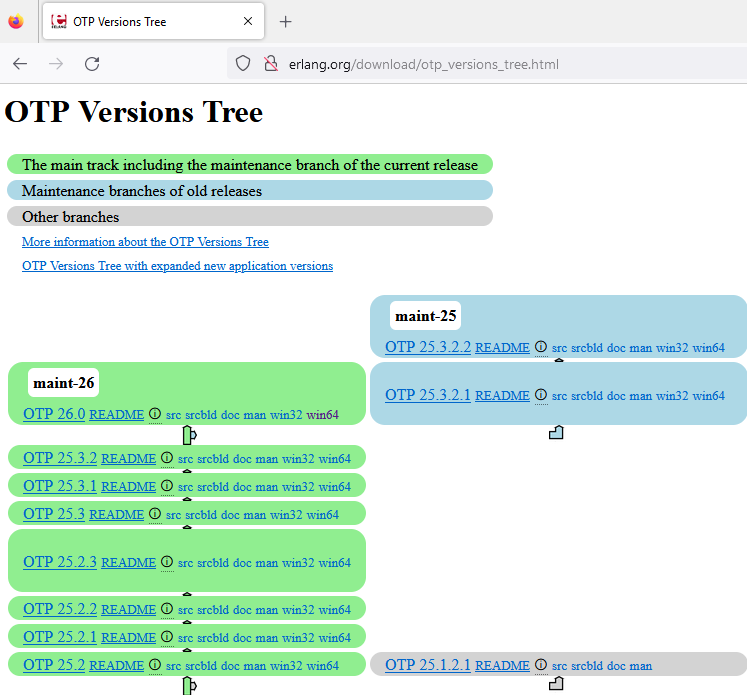
\includegraphics[width=1\textwidth]{figures/fig1.png}
\caption{Strona internetowa, z której można pobrać erlang.}
\label{fig:zdjecie}
\end{figure}


Po procesie instalacji, należało dodać Zmienną środowiskową (którą można znaleźć w zaawansowanych właściwościach systemu).

\begin{figure}[!htb]
	\centering
	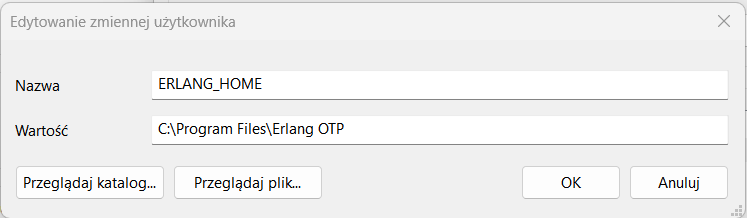
\includegraphics[width=0.9\textwidth]{figures/fig2.png}
	\caption{Dodana zmienna środowiskowa.}
	\label{fig:fig2}
\end{figure}

Po jej dodaniu, zmienne środowiskowe wyglądały następująco:

\begin{figure}[!htb]
	\centering
	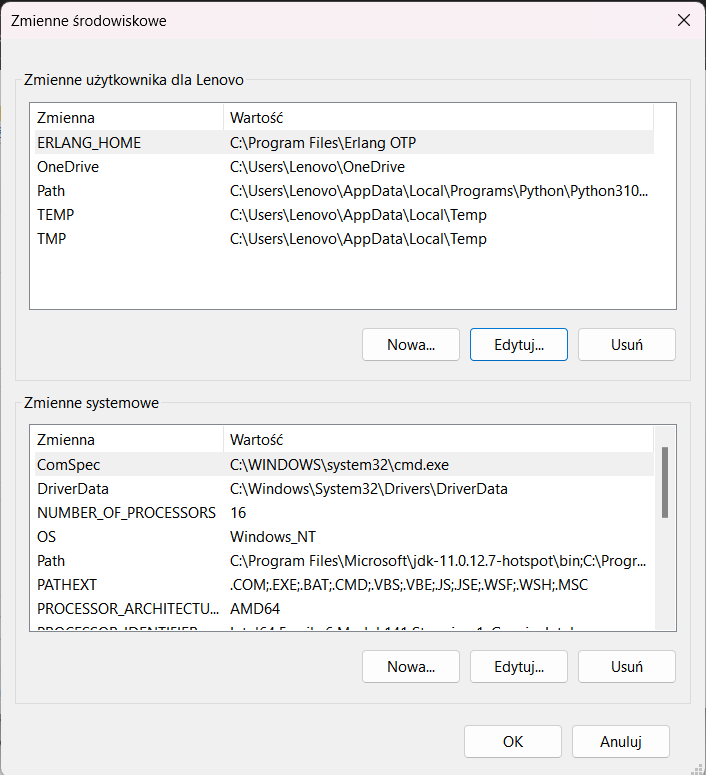
\includegraphics[width=0.75\textwidth]{figures/fig3.png}
	\caption{Zmienne środowiskowe.}
	\label{fig:fig3}
\end{figure}

Następnie, po sprawdzeniu w CMD dodanej zmiennej środowiskowej otrzymujemy jej ścieżkę, oznacza to, że wszystko przebiegło pomyślnie.

\begin{figure}[!htb]
	\centering
	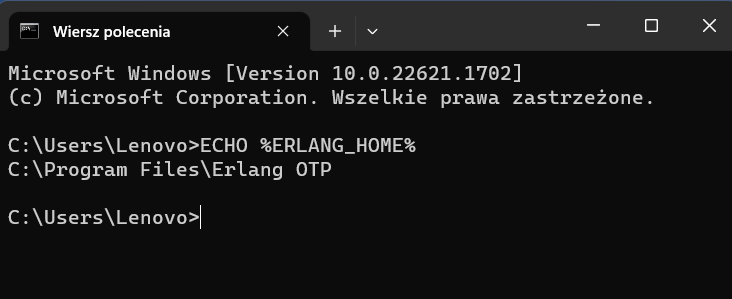
\includegraphics[width=0.7\textwidth]{figures/fig4.png}
	\caption{Sprawdzenie w CMD.}
	\label{fig:fig4}
\end{figure}

\subsection{RabbitMQ}
Należało pobrać \href{https://github.com/rabbitmq/rabbitmq-server/}{RabbitMQ} ze strony github, a następnie zainstalować.\\
Po udanej instalacji, trzeba było otworzyć wiersz poleceń z uprawnieniami administratora, a następnie wejść w ścieżkę nowo pobranego programu. Jako że przy poprzednich próbach był problem z uruchomieniem \textit{rabbitmq-server.bat}, należało użyć polecenia \textit{rabbitmq plugins enable rabbitmq management}, które pozwoliło na dostęp do wtyczek. \\
Wtyczki, które zostały włączone to: \textit{rabbitmq management, rabbitmq management agent} oraz \textit{rabbitmq web dispatch}. 

\begin{figure}[!htb]
	\centering
	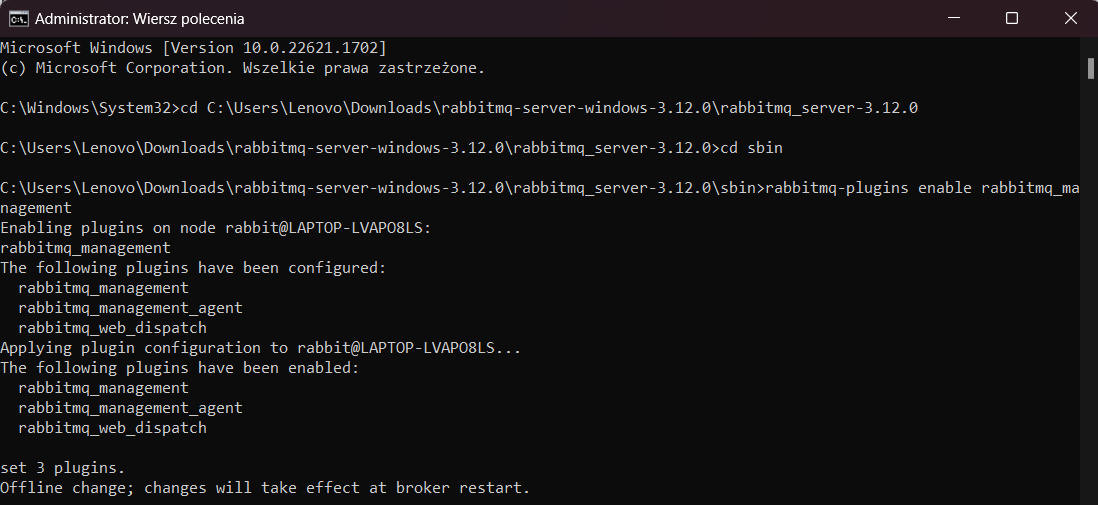
\includegraphics[width=1\textwidth]{figures/fig5.png}
	\caption{Pozwolenie na dostęp do wtyczek.}
	\label{fig:fig5}
\end{figure}
\clearpage

Następnie uruchomiono RabbitMQ używając polecenia \textit{rabbitmq-server.bat}:
\begin{figure}[!htb]
	\centering
	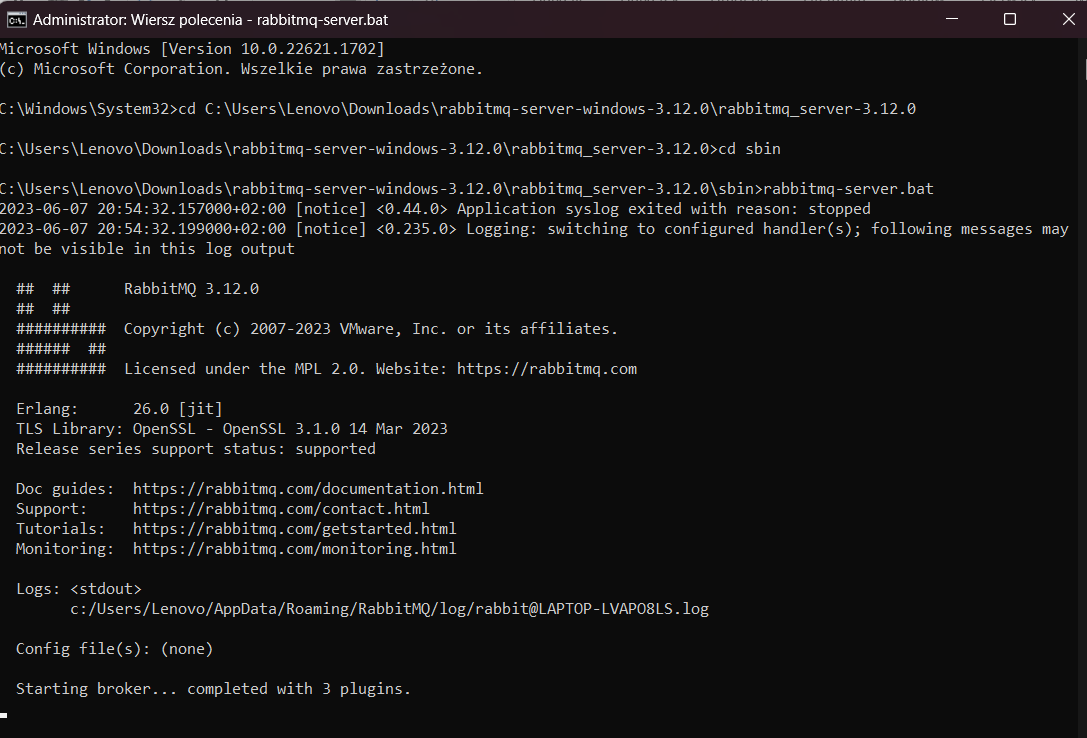
\includegraphics[width=1\textwidth]{figures/fig6.png}
	\caption{Uruchomienie brokera.}
	\label{fig:zdjecie}
\end{figure}

Wszystko przebiegło pomyślnie biorąc pod uwagę fakt, że jest podana informacja o 3 załadowanych wtyczkach.\\
Dodatkowo, po uruchomieniu \textit{localhost:15672} w przegląrdarce, otrzymano:
\begin{figure}[!htb]
	\centering
	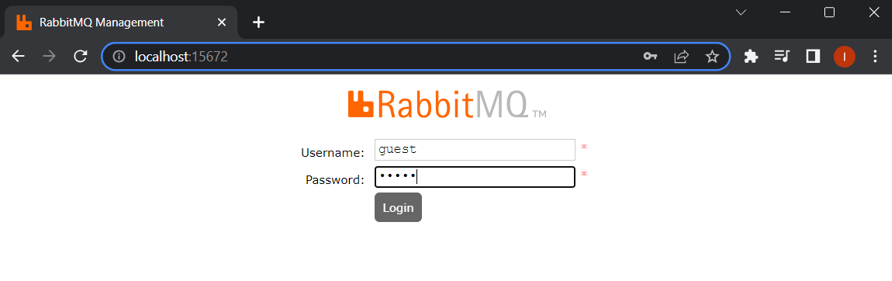
\includegraphics[width=1\textwidth]{figures/fig7.png}
	\caption{Logowanie do RabbitMQ.}
	\label{fig:zdjecie}
\end{figure}
\clearpage

Po zalogowaniu się otrzymujemy:
\begin{figure}[!htb]
	\centering
	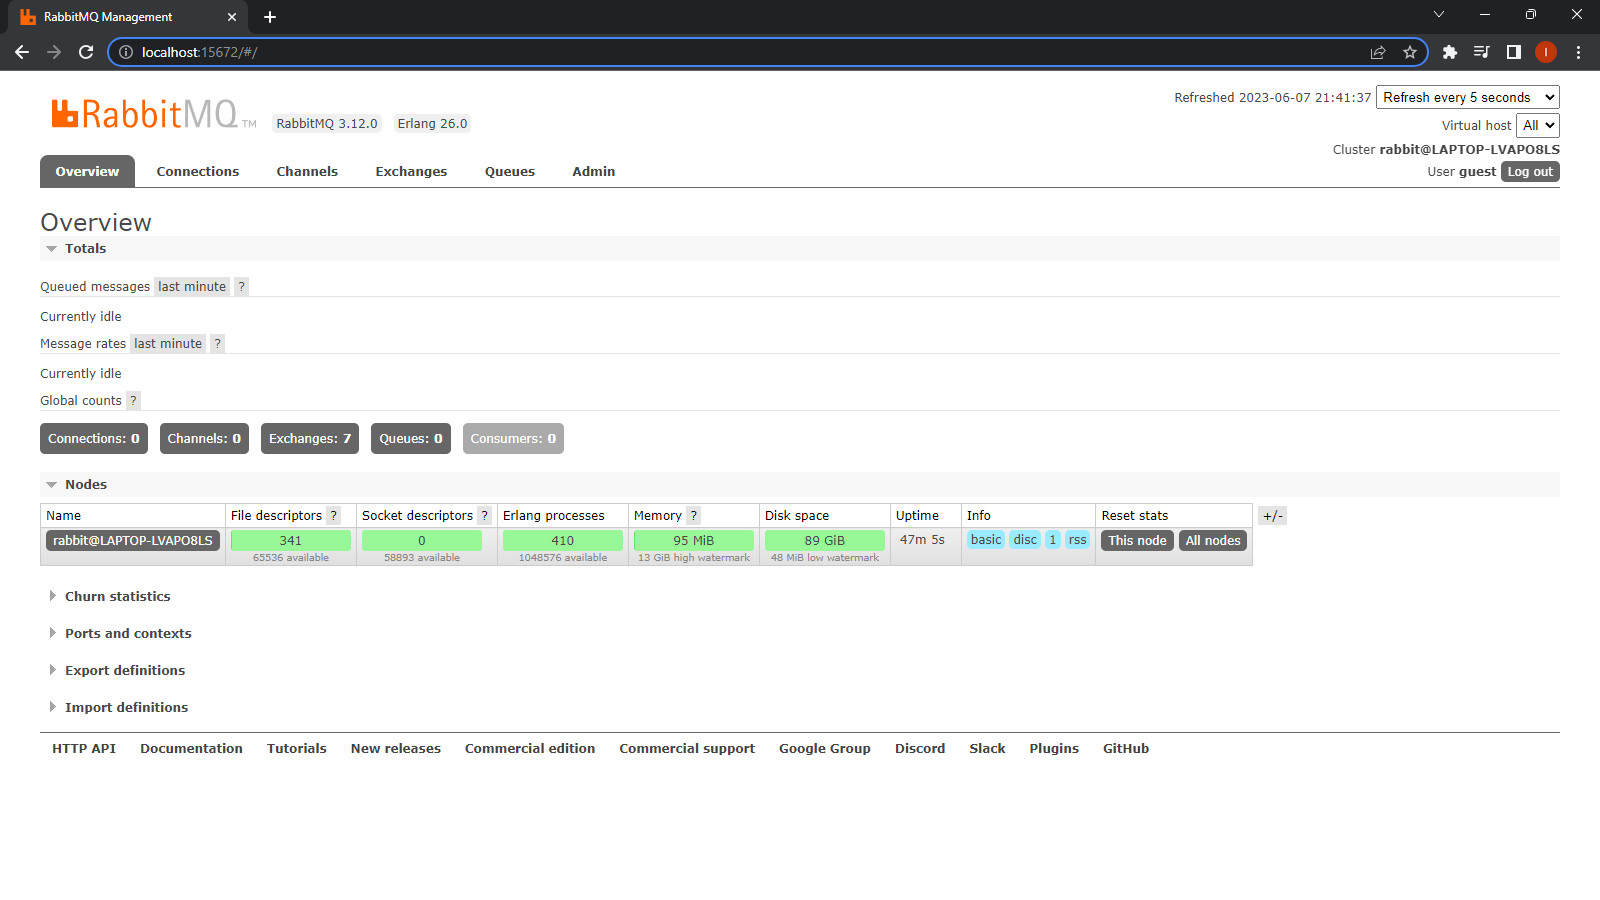
\includegraphics[width=1\textwidth]{figures/fig8.png}
	\caption{Strona RabbitMQ.}
	\label{fig:zdjecie}
\end{figure}

\section{Projekt}
\subsection{Alternatywna wymiana i wymiana dead-letter}
Alternatywna wymiana to mechanizm umożliwiający przekierowanie wiadomości, które nie mogą zostać dostarczone do ich docelowej kolejki. Gdy wiadomość nie może zostać dostarczona do żadnej kolejki związaną bezpośrednio z daną wymianą, RabbitMQ przekierowuje tę wiadomość do alternatywnej wymiany (alternate exchange).
\clearpage

\begin{figure}[!htb]
	\centering
	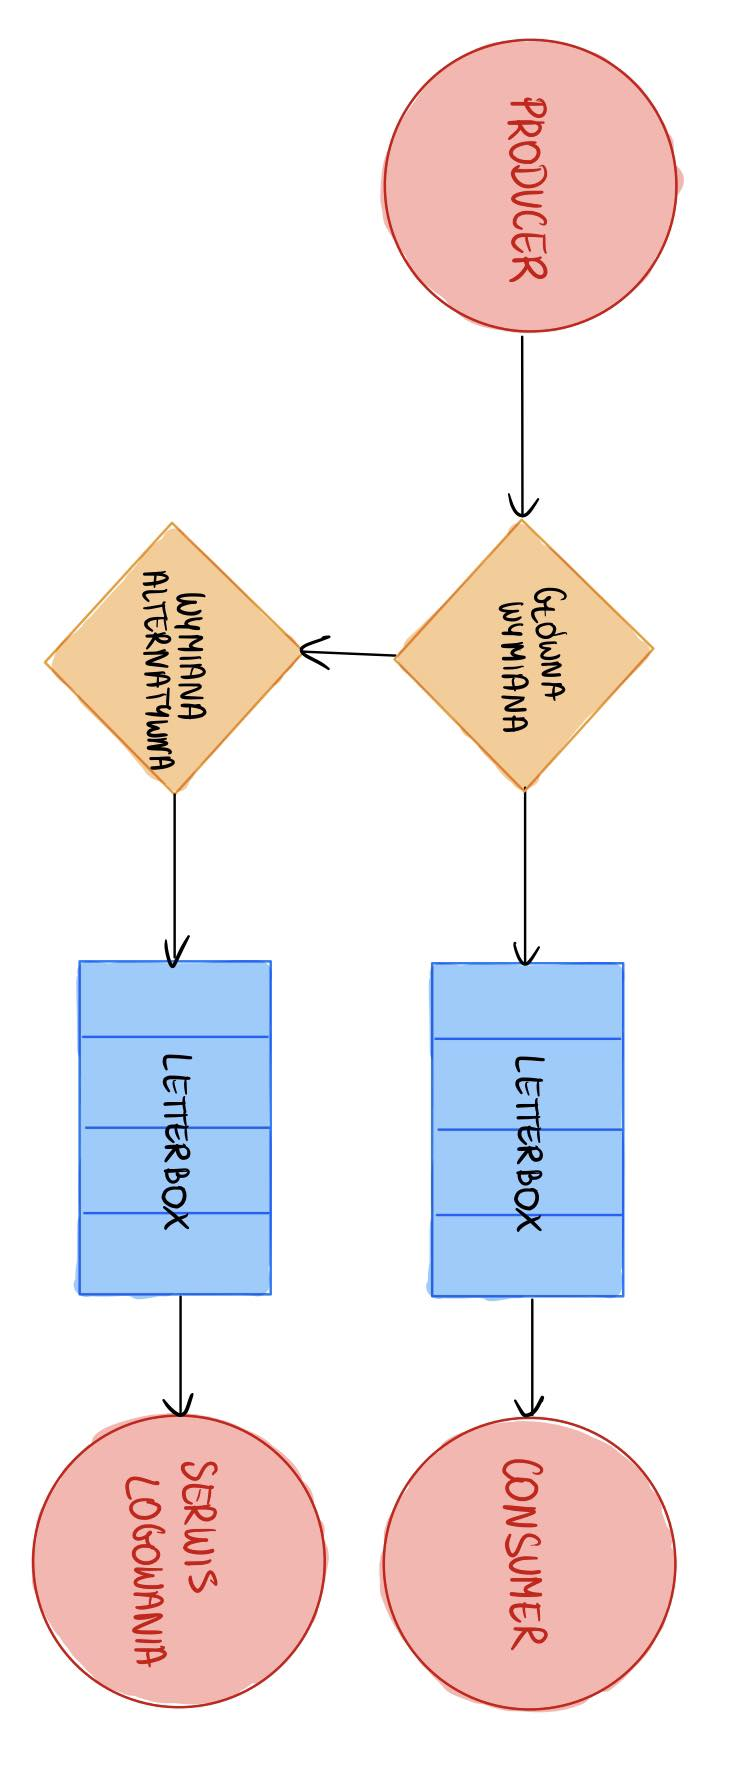
\includegraphics[angle=90,width=1\textwidth]{figures/fig10.png}
	\caption{Alternatywna wymiana.}
	\label{fig:zdjecie}
\end{figure}

Wymiana kolejki martwej jest specjalnym rodzajem wymiany, która służy do przekierowywania wiadomości, które nie mogą być przetworzone przez ich pierwotną kolejkę. Gdy wiadomość zostaje oznaczona jako "umieszczona w kolejkę martwą" (ang. dead-lettered), jest przekierowywana do wymiany "dead-letter", gdzie może być dalej przetwarzana lub analizowana.

\begin{figure}[!htb]
	\centering
	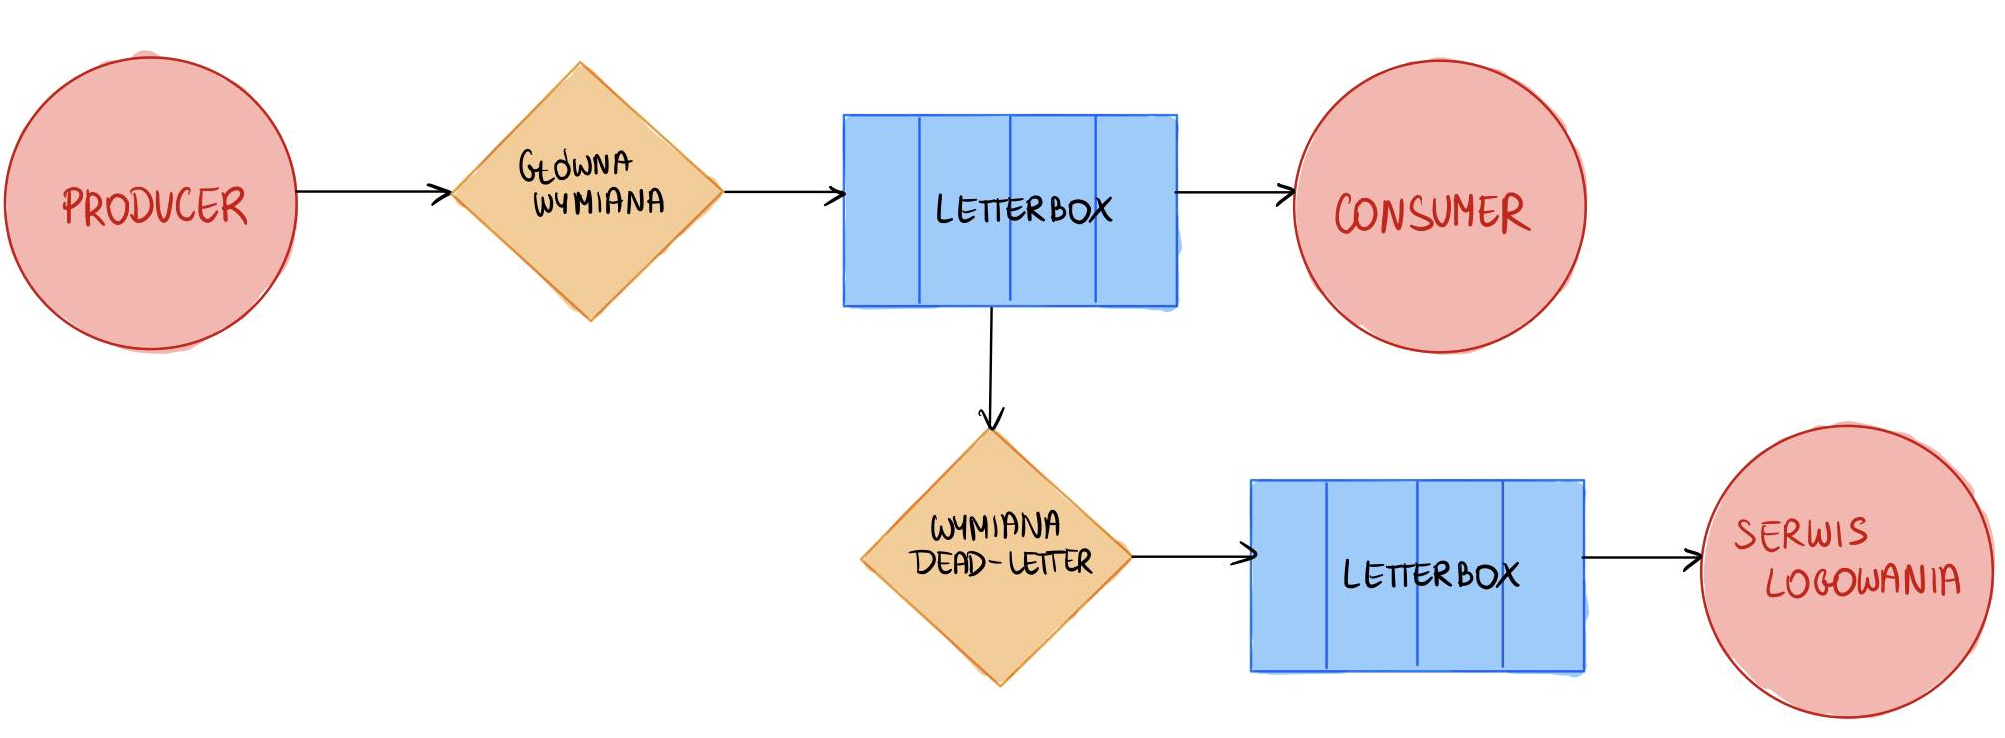
\includegraphics[width=1\textwidth]{figures/fig11.png}
	\caption{Wymiana kolejki martwej.}
	\label{fig:zdjecie}
\end{figure}
\clearpage

Postanowiłam połączyć te dwie wymiany, w wyniku czego stworzyłam następujący kod dla konsumera  (consumer):


\begin{figure}[!htb]
	\centering
	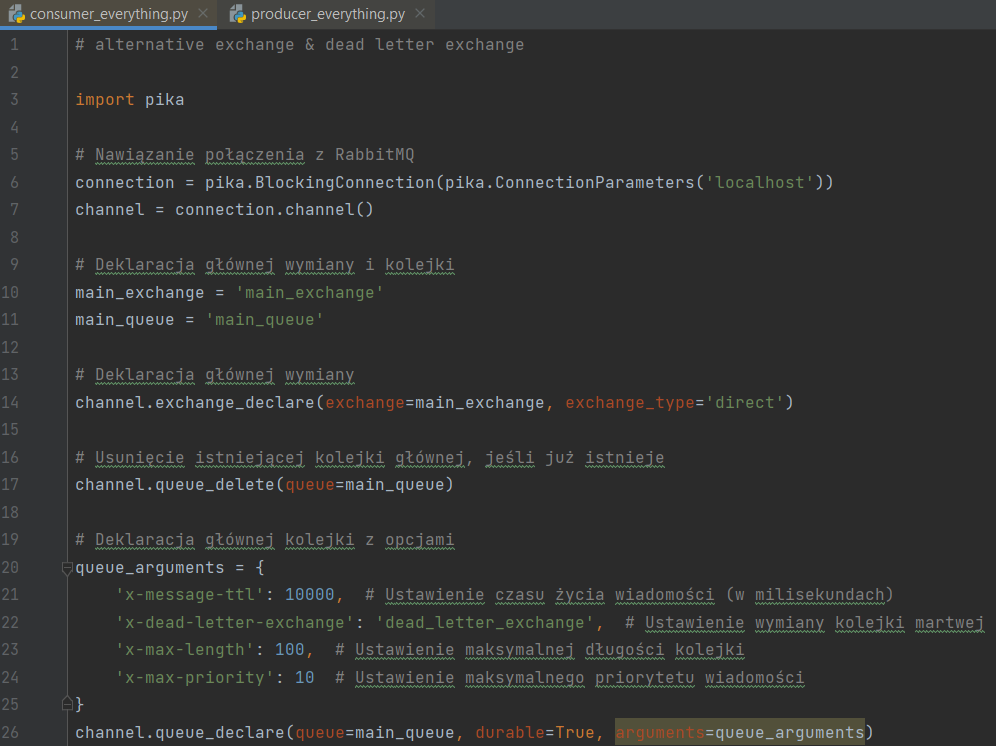
\includegraphics[width=1\textwidth]{figures/fig12}
	\caption{Consumer - wymiana alternatywna i kolejki martwej, część 1.}
	\label{fig:zdjecie}
\end{figure}

\begin{figure}[!htb]
	\centering
	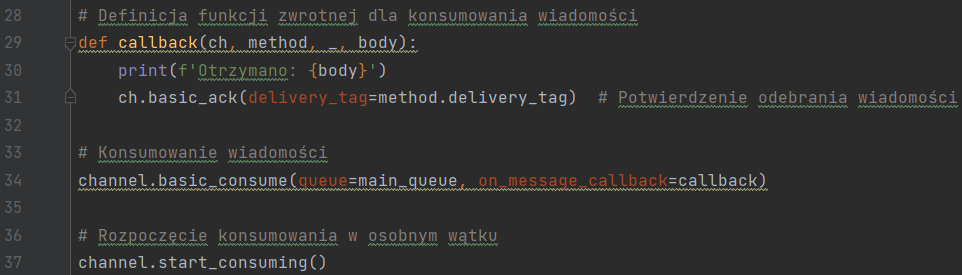
\includegraphics[width=1\textwidth]{figures/fig13}
	\caption{Consumer - wymiana alternatywna i kolejki martwej, część 2.}
	\label{fig:zdjecie}
\end{figure}

Celem tego kodu jest utworzenie prostego programu konsumera w RabbitMQ. Program ten ma za zadanie połączyć się z lokalnym serwerem RabbitMQ, zadeklarować wymianę i kolejkę, skonfigurować odpowiednie opcje dla kolejki, skonsumować wiadomości z kolejki oraz przetworzyć je przy użyciu określonej funkcji zwrotnej. 

Następujący kod konsumera po kolei:
\begin{enumerate}[label=\arabic*), leftmargin=1.25cm]
	\item Nawiązuje połączenie z lokalnym serwerem RabbitMQ.
	\item Deklaruje wymianę o nazwie \textit{main exchange} typu \textit{direct}.
	\item Usuwa istniejącą kolejkę o nazwie \textit{main queue}, jeśli taka istnieje.
	\item Deklaruje kolejkę o nazwie \textit{main queue} z określonymi opcjami, takimi jak czas życia wiadomości, wymiana kolejki martwej, maksymalna długość kolejki i maksymalny priorytet wiadomości.
	\item Definiuje funkcję zwrotną callback, która jest wywoływana przy odbiorze wiadomości z kolejki.
	\item Konsumuje wiadomości z kolejki \textit{main queue}, wywołując funkcję zwrotną callback dla każdej otrzymanej wiadomości.
	\item Rozpoczyna proces konsumowania wiadomości w osobnym wątku.
	\item Zamyka połączenie z RabbitMQ po zakończeniu konsumowania.
\end{enumerate}
\clearpage

Natomiast niżej jest przedstawiony kod dla producenta:

\begin{figure}[!htb]
	\centering
	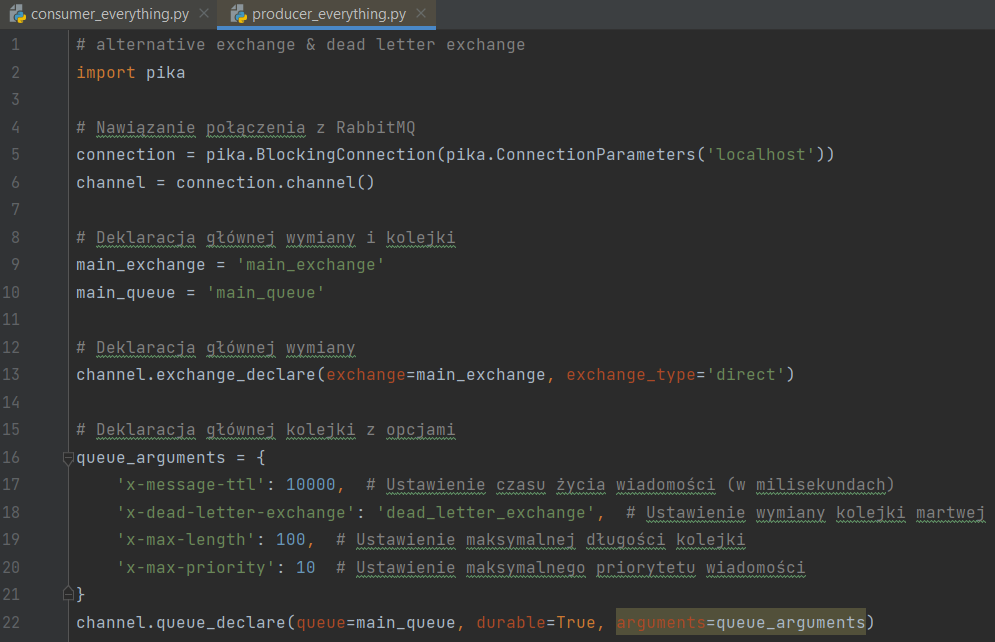
\includegraphics[width=1\textwidth]{figures/fig14}
	\caption{Producer - wymiana alternatywna i kolejki martwej, część 1.}
	\label{fig:zdjecie}
\end{figure}

\begin{figure}[!htb]
	\centering
	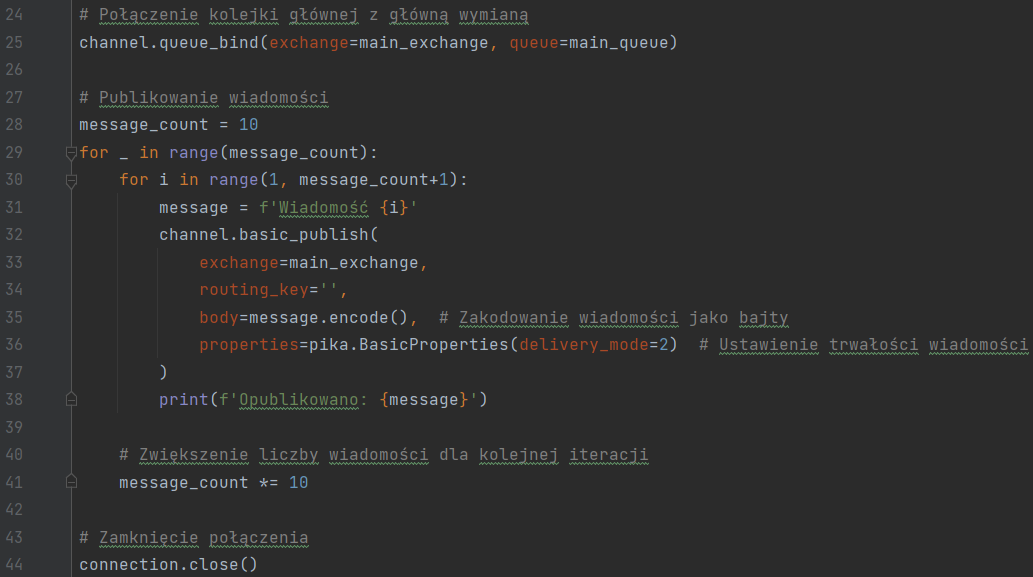
\includegraphics[width=1\textwidth]{figures/fig15}
	\caption{Producer - wymiana alternatywna i kolejki martwej, część 2.}
	\label{fig:zdjecie}
\end{figure}

Celem tego kodu jest zaprezentowanie przykładu użycia mechanizmów alternatywnej wymiany oraz kolejki martwej  w RabbitMQ. Kod tworzy główną wymianę, kolejkę i publikuje wiadomości, które są przetwarzane zgodnie z zdefiniowanymi opcjami, takimi jak czas życia wiadomości, priorytet i maksymalna długość kolejki. Wykorzystanie alternatywnej wymiany pozwala na przekierowanie wiadomości, które nie mogą zostać dostarczone do głównej kolejki, do innej wymiany. Natomiast ustawienie kolejki martwej umożliwia przechwycenie wiadomości, które nie mogą zostać obsłużone przez główną kolejkę, umożliwiając dalsze przetwarzanie lub analizę takich wiadomości.


Następujący kod konsumera po kolei:
\begin{enumerate}[label=\arabic*), leftmargin=1.25cm]
	\item Nawiązuje połączenie z serwerem RabbitMQ.
	\item Deklaruje wymianę o nazwie \textit{main exchange} typu \textit{direct}.
	\item Deklaruje kolejkę o nazwie \textit{main queue} z określonymi opcjami, takimi jak czas życia wiadomości, wymiana kolejki martwej, maksymalna długość kolejki i maksymalny priorytet wiadomości.
	\item Łączy kolejkę \textit{main queue} z wymianą \textit{main exchange}.
	\item Publikuje wiadomości do wymiany \textit{main exchange} o różnych treściach i priorytetach.
	\item Liczba wiadomości, które są publikowane, jest iteracyjnie zwiększana, aby zobaczyć wpływ na kolejkę.
	\item Każda wiadomość jest kodowana jako bajty i ustawiana jako trwała, aby przetrwała restart serwera RabbitMQ.
	\item Wyświetla informacje o opublikowanych wiadomościach.
	\item Po zakończeniu publikowania, zamyka połączenie z RabbitMQ.
\end{enumerate}

\clearpage

Po uruchomieniu powyższego kodu możemy skorzystać z poniższych przycisków w RabbitMQ.
\begin{figure}[!htb]
	\centering
	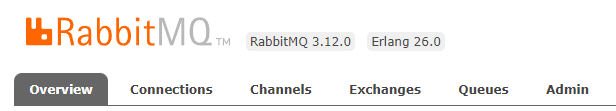
\includegraphics[width=1\textwidth]{figures/fig21}
	\caption{Menu RabbitMQ.}
	\label{fig:zdjecie}
\end{figure}

Po wybraniu "connections" otrzymujemy tabelkę widoczną poniżej. Można tu zauważyć połączenia z konsumerem, jak i z producerem.
\begin{figure}[!htb]
	\centering
	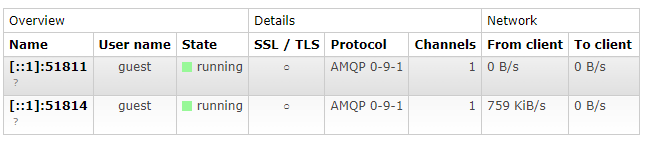
\includegraphics[width=0.9\textwidth]{figures/fig16}
	\caption{Widoczne połączenia (connections) w RabbitMQ.}
	\label{fig:zdjecie}
\end{figure}


Po wybraniu "channels" otrzymujemy tabelkę widoczną poniżej. Wynika z tego, że kanał 51811 (połączenie z konsumerem) jest bezczynny, czyli nie wykonuje żadnych operacji i czeka. Z kolei kanał 51814 (związany z producerem) jest aktywny i wszystkie wiadomości, które wysyła są usuwane.
\begin{figure}[!htb]
	\centering
	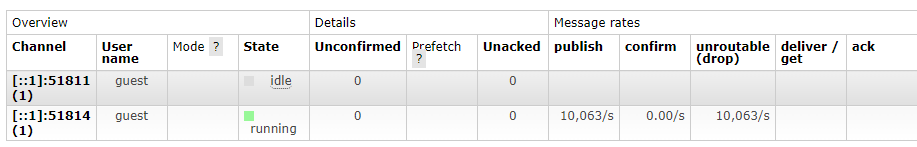
\includegraphics[width=1\textwidth]{figures/fig17}
	\caption{Widoczne kanały (channels) w RabbitMQ.}
	\label{fig:zdjecie}
\end{figure}
\clearpage

Po wybraniu "exchanges" otrzymujemy poniższą tabelkę. Wynika z niej, że wszystkie wymiany idą do \textit{main exchange}.
\begin{figure}[!htb]
	\centering
	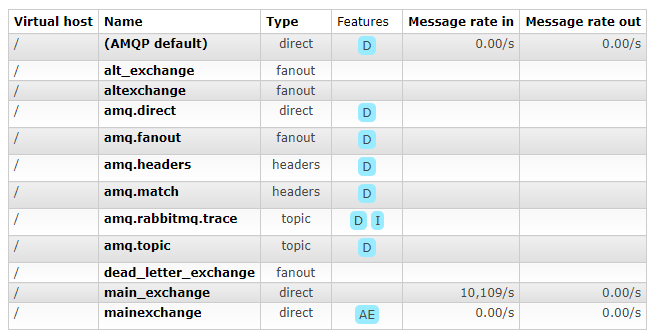
\includegraphics[width=1\textwidth]{figures/fig18}
	\caption{Widoczne wymiany (exchanges) w  RabbitMQ.}
	\label{fig:zdjecie}
\end{figure}


Po wejściu w połączenie z konsumerem po paru minutach otrzymujemy poniższy wykres. Na początku połączenia jest widoczna większa aktywność, natomiast później widoczna jest bezczynność.
\begin{figure}[!htb]
	\centering
	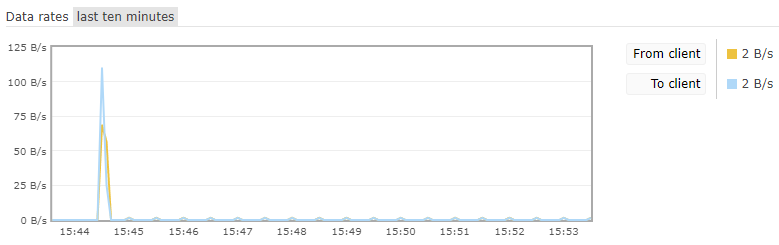
\includegraphics[width=1\textwidth]{figures/fig19}
	\caption{Wykres połączenia konsumera z RabbitMQ.}
	\label{fig:zdjecie}
\end{figure}
\clearpage


Natomiast po wejściu w połączenie z producerem po paru minutach otrzymujemy wykres widoczny poniżej. Na tym wykresie jest widoczny duży przesył wiadomości, który się utrzymuje na podobnym poziomie, a po jakimś czasie zmniejsza się.
\begin{figure}[!htb]
	\centering
	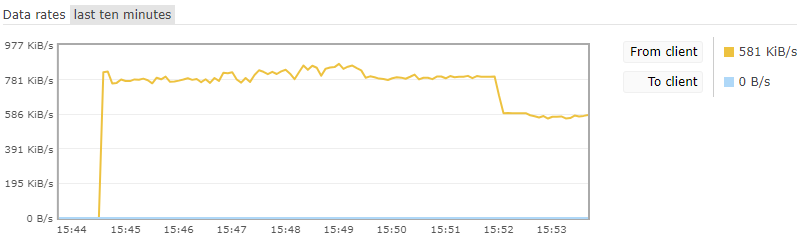
\includegraphics[width=1\textwidth]{figures/fig20}
	\caption{Wykres połączenia producera z RabbitMQ.}
	\label{fig:zdjecie}
\end{figure}



\clearpage
\addcontentsline{toc}{section}{Bibliografia}

\begin{thebibliography}{4}
\bibitem{str} http://weii.portal.prz.edu.pl/pl/materialy-do-pobrania
\bibitem{Strona domowa RabbitMQ} https://www.rabbitmq.com/
\bibitem{Dokumentacja RabbitMQ} https://www.rabbitmq.com/documentation.html
\bibitem{Oficjalne repozytorium GitHub RabbitMQ} https://github.com/rabbitmq/rabbitmq-server
\bibitem{Wymiana dead-letter} https://www.rabbitmq.com/dlx.html
\bibitem{Wymiana alternatywna} https://www.rabbitmq.com/ae.html
\end{thebibliography}

\clearpage



\end{document} 
